\chapter{Implementation}\label{ch:C}
\section{Design process}
UX/UI design is one of the earliest and the most important stages of building a successful project. To make it more conscious and consistent, we started from market and user researches using methods such as survey, analysis of analogues, user stories and user personas. The goal was to answer questions:

- What problem do your users need solving?

- What are their behaviors, needs and motivations?
Finally on this stage, we formed two user personas that approximately describe future ordinary users of the website. (See Figure \ref{fig:image001}, \ref{fig:image003}).
\begin{figure}[h]
    \centering
    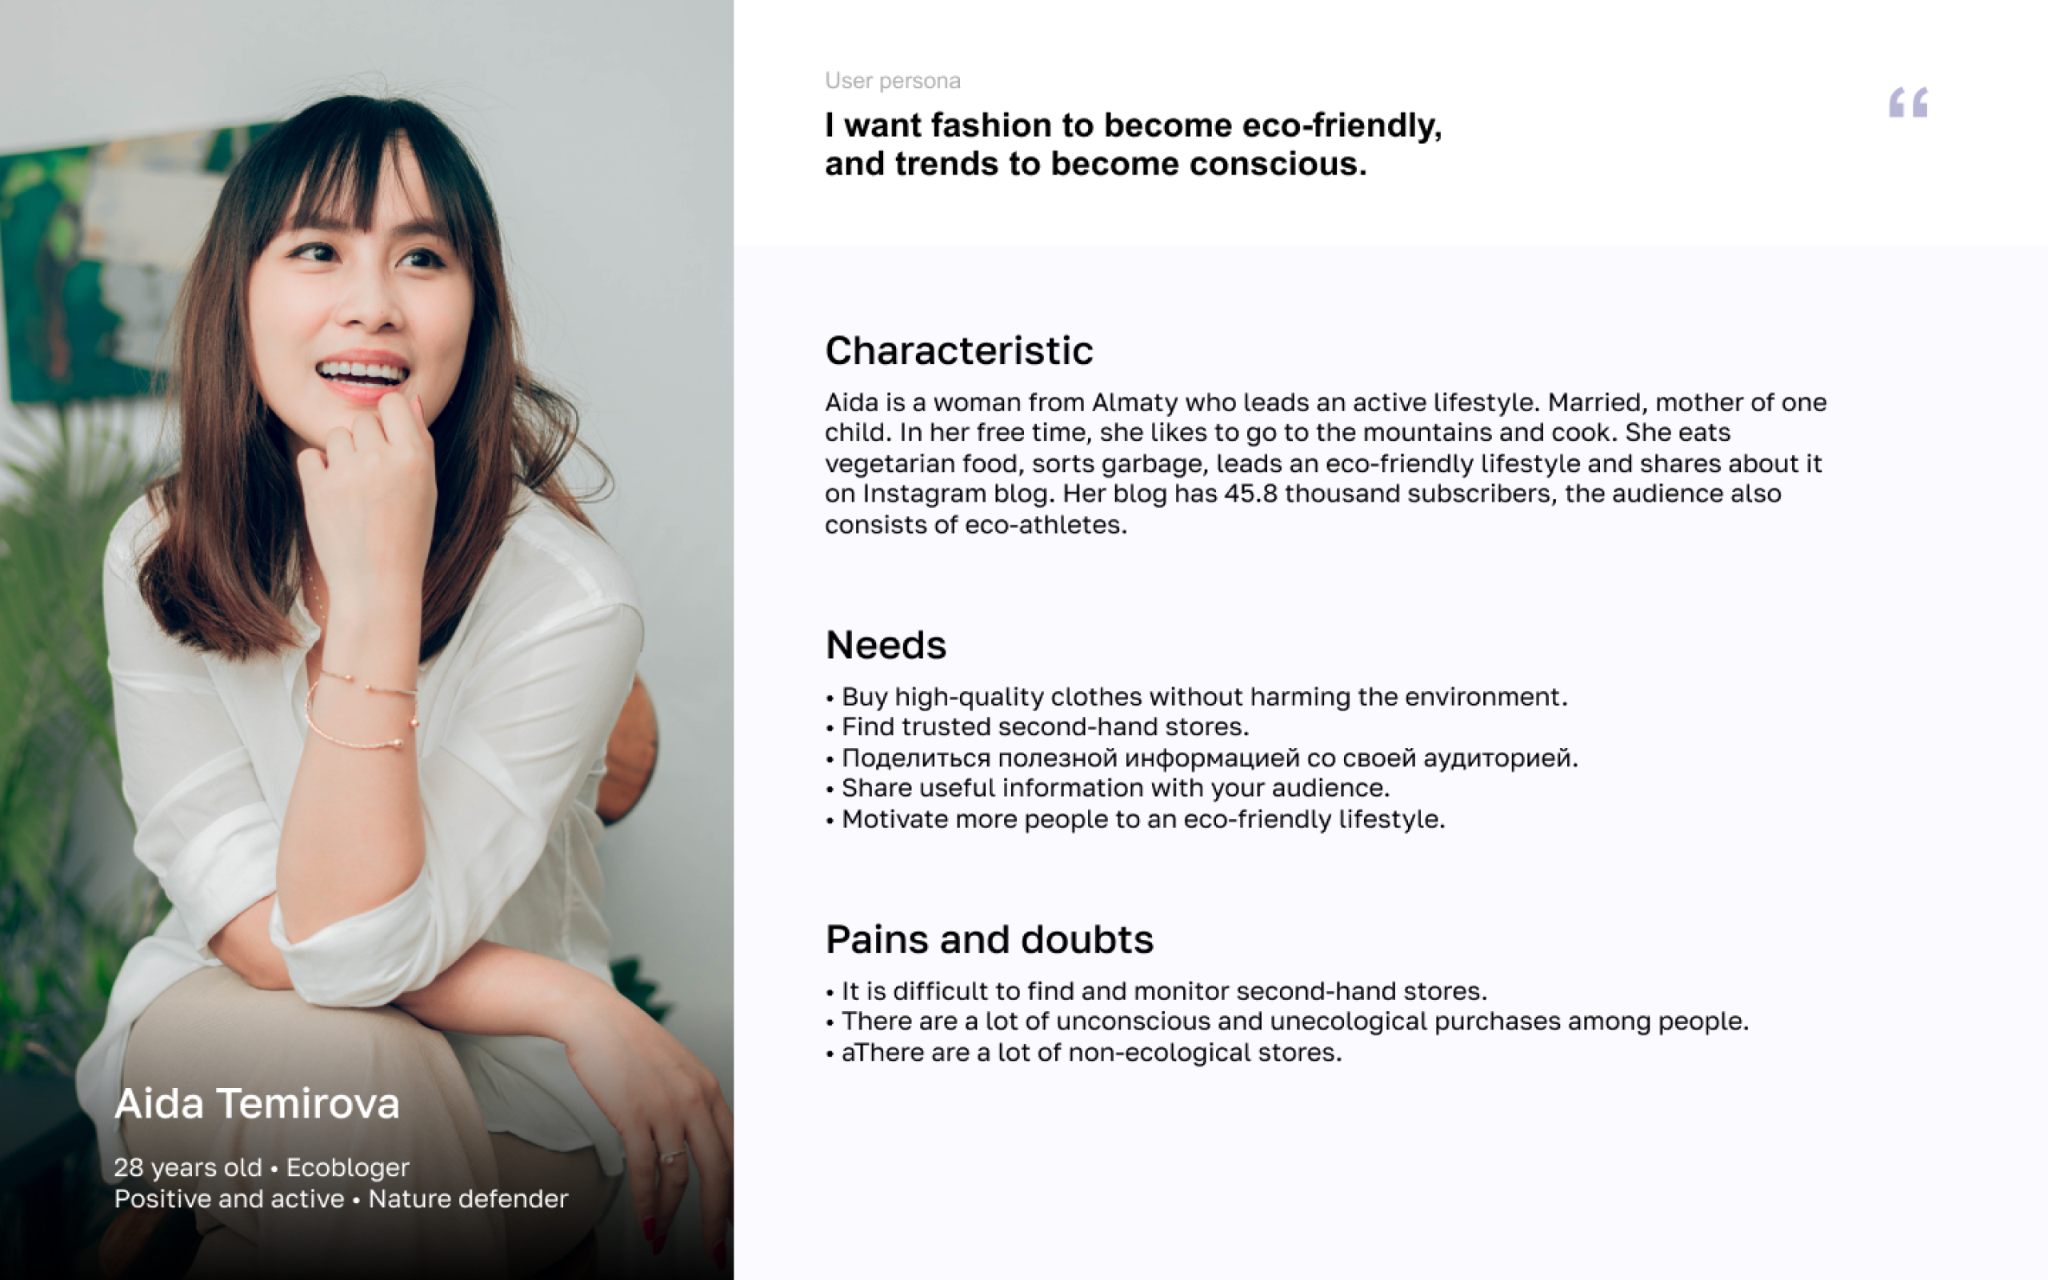
\includegraphics[scale=0.22]{figures/image001.png}
    \caption{user personas}
    \label{fig:image001}
\end{figure}
\begin{figure}[t!]
    \centering
    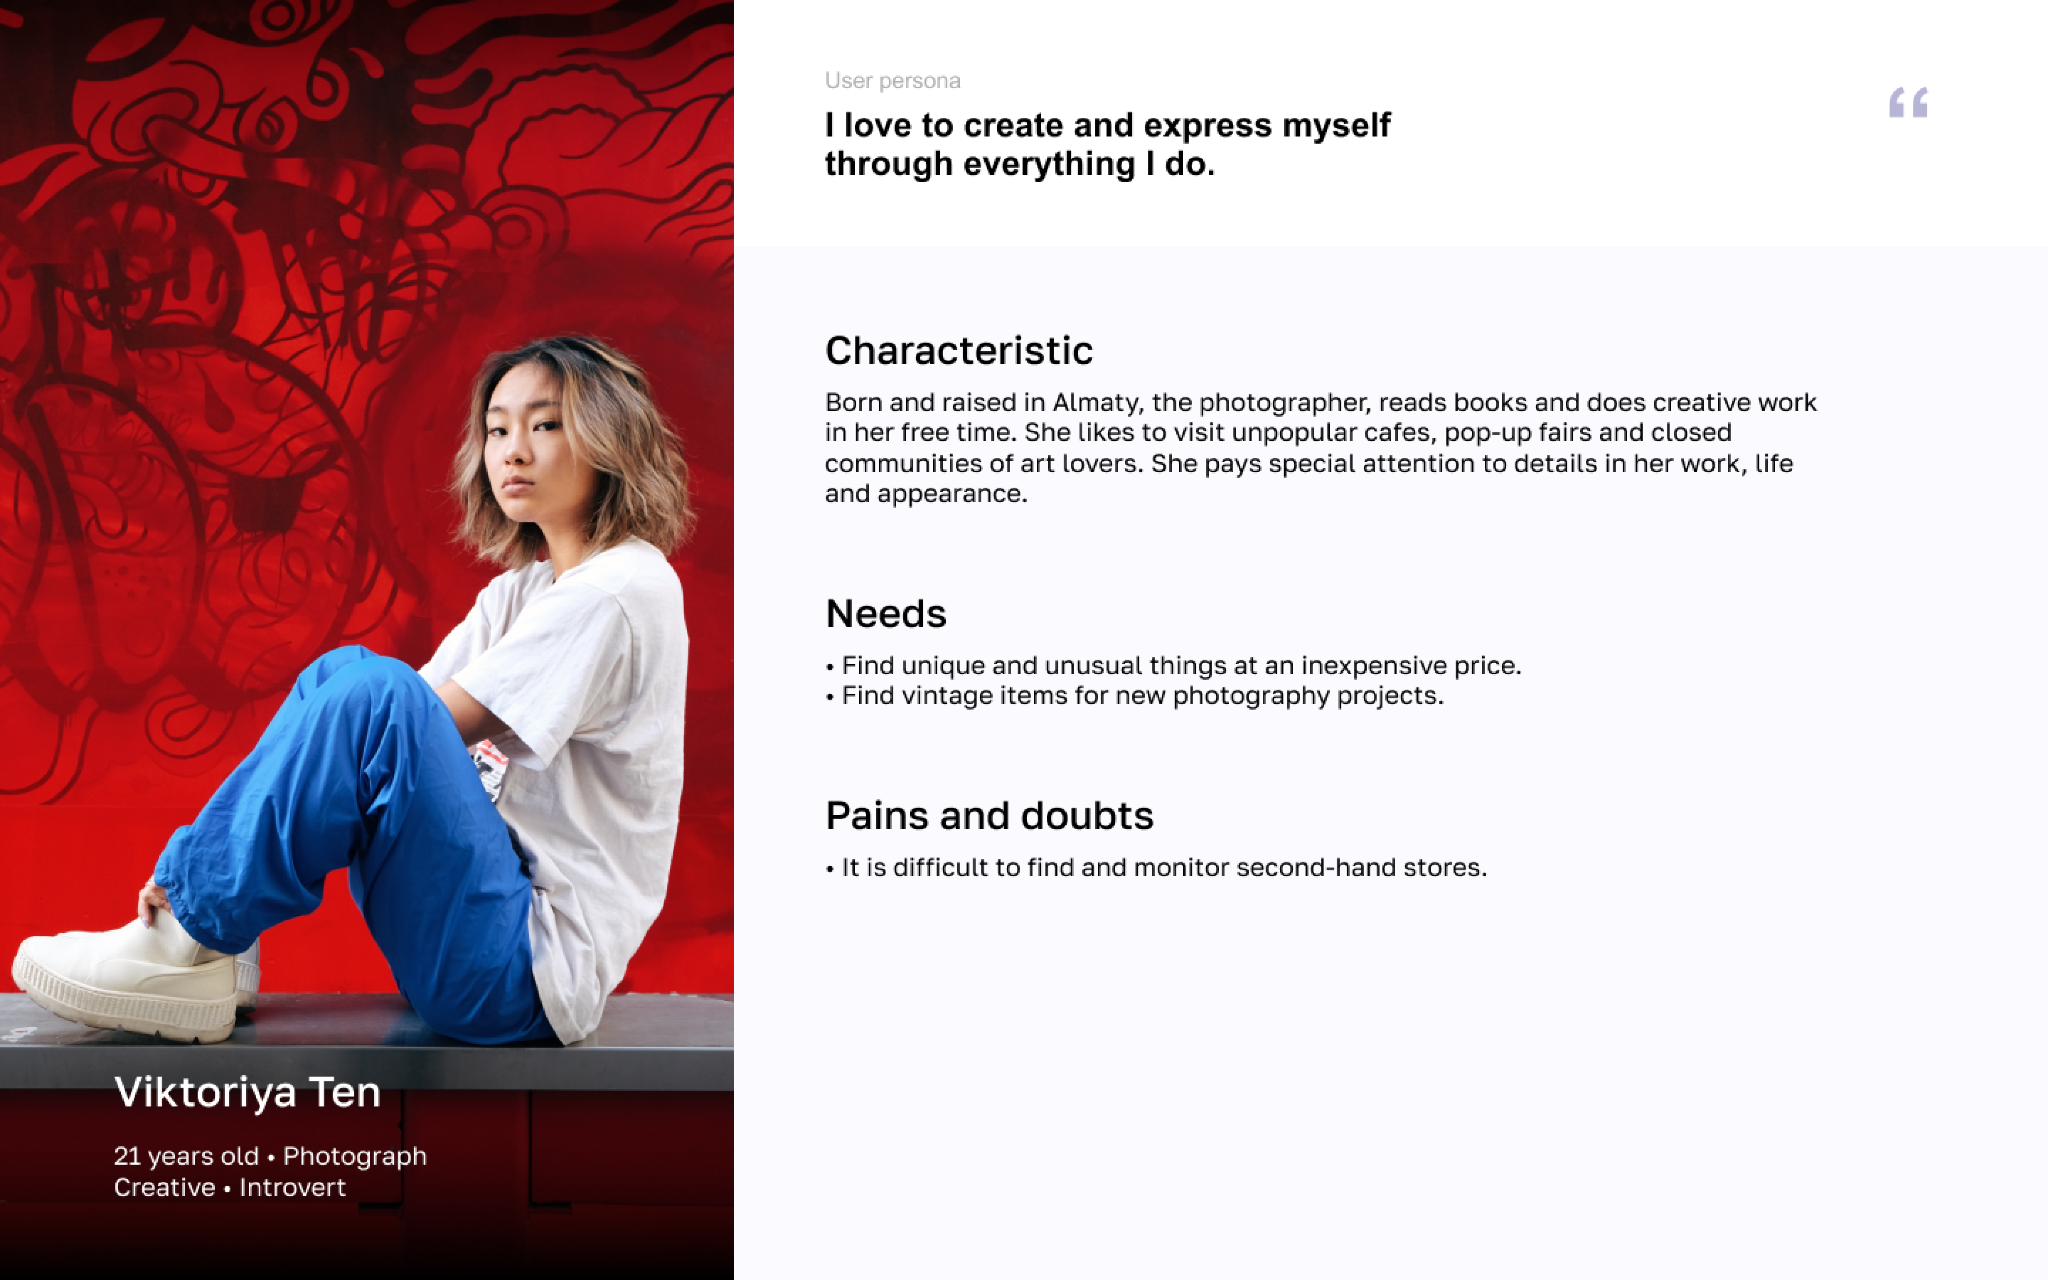
\includegraphics[scale=0.22]{figures/image003.png}
    \caption{user personas}
    \label{fig:image003}
\end{figure}

After understanding what aspects should be considered, we moved to the next step: Information Architecture. It’s a part of the UX process, where the hierarchy, navigation and structure of the visual part of the website are described. The scheme was constructed on the tool Miro. Design was separated for two roles: customer and shop owner.
Website structure for customer consists of: 

- Main page (main banner, main categories of products, auction of the day, products with sale, shops)

- Catalog (categories and subcategories, and clothes itself)

- Auctions (clothes on the auction)

- Shops

- Profile (personal information and orders journal)
Authorization\\

While for the shop owner:

- Authorization

- Dashboard (analytics)

- Catalog (Add, delete and edit products)

- Orders

- Shop (Editing information about shop)

The next stage was Designing Wireframes, which started from drawing simple prototypes abstractly showing location of each element and finishing with high fidelity wireframes grouped into flows(Our full design in Appendix \ref{app:A}). Figma was the most convenient tool for implementing this task, because it gives opportunity to make work more effective and consistent. (See Figure \ref{fig:image005},\ref{fig:image007}).

\begin{figure}[h]
    \centering
    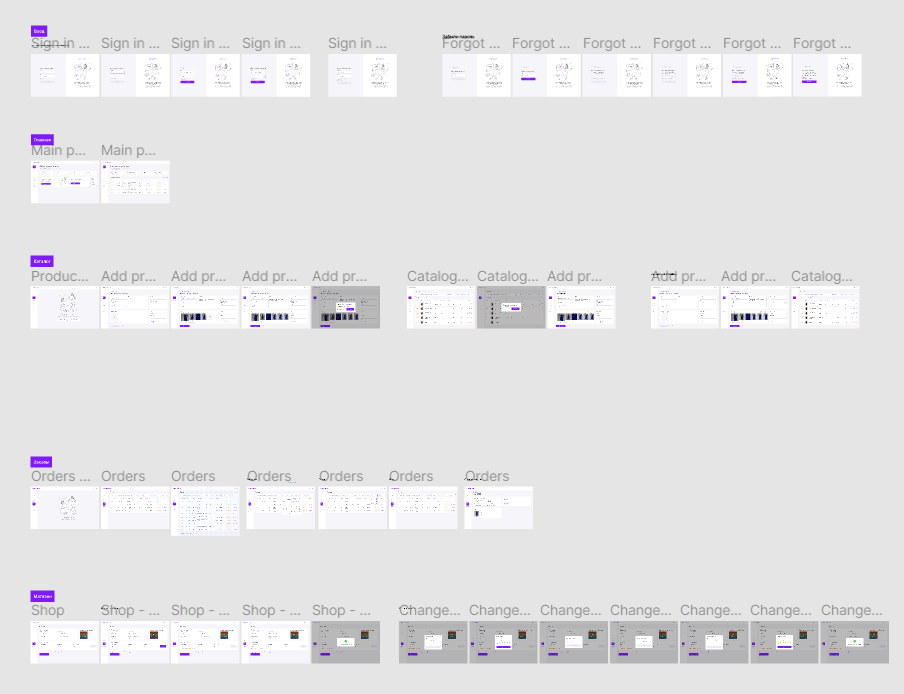
\includegraphics[scale=0.53]{figures/image005.png}
    \caption{Wireframes for shop owner}
    \label{fig:image005}
\end{figure}
\begin{figure}[pt!]
    \centering
    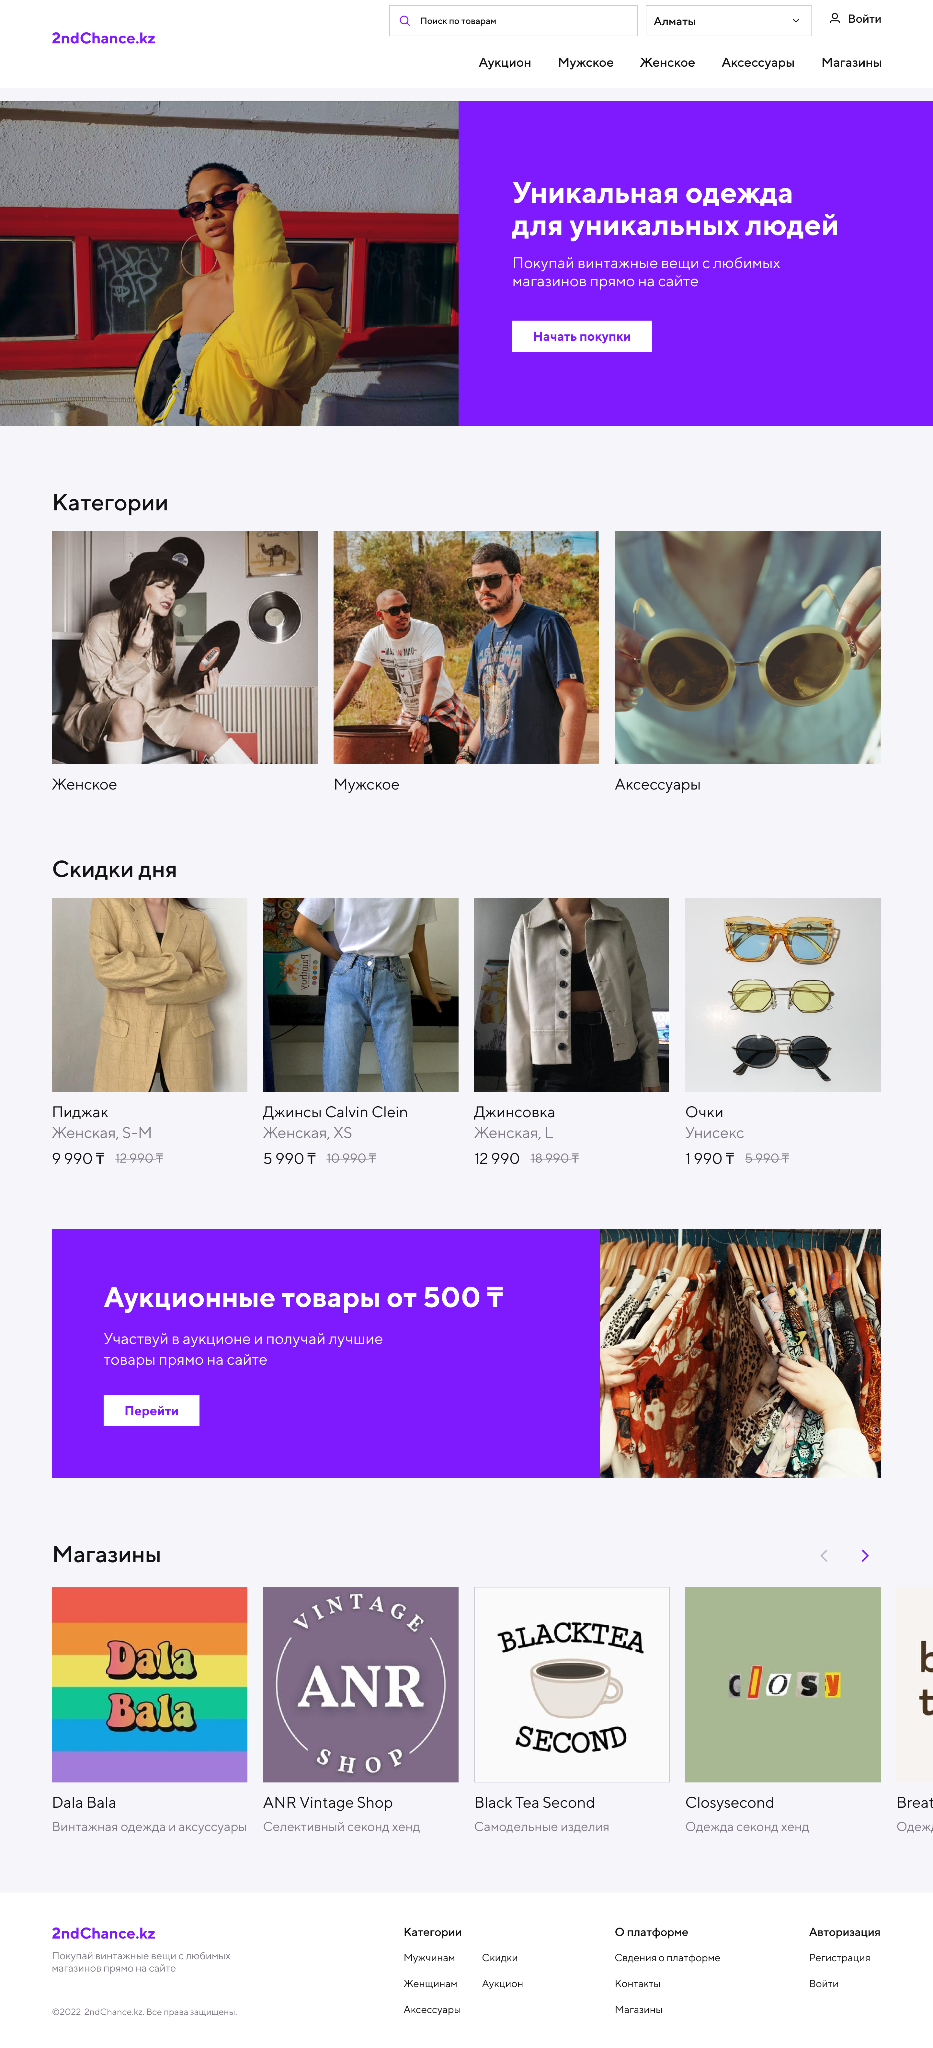
\includegraphics[scale=0.33]{figures/image007.png}
    \caption{Client main page}
    \label{fig:image007}
\end{figure}
\clearpage
%Monkey is a beast that can jump. See Appendix \ref{app:B}.
\section{Project database}
There are many dbms (database management systems) to raise the database but our choice was
postgres\cite{greenpeace} because of its great advantages. (See Figure \ref{fig:database}).
\begin{figure}[ht!]
    \centering
    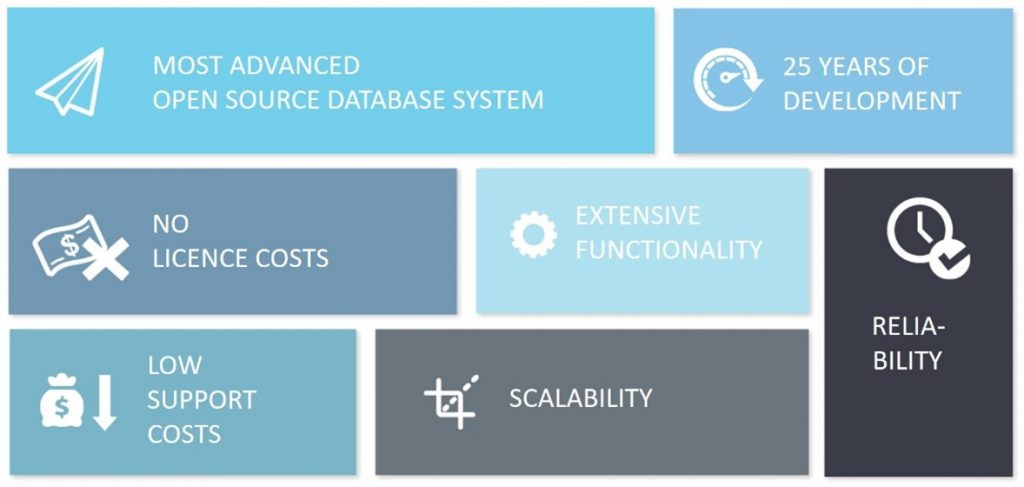
\includegraphics[scale=0.5]{figures/database.jpg}
    \caption{Advantages of postgres}
    \label{fig:database}
\end{figure}

However not all the features are used in our project, it is still the most comfortable dbms
and for more convenient data management, it was decided to make it remote, due to free
service heroku.

Although postgres is nice place to save data\cite{postgre}, in our project there is an auction
functionality and using just simple dbms would not be enough to meet the response speed
requirements. Therefore we used redis rdbms. Since no/sql languages   have an advantage over
just sql languages   for example data processing speed, scalability, distributed systems

Also to run our web site on a server we used ngrok for its simplicity and convenience
As a server we used Raspberry Pi because of its low cost, processing power, linux support, many
interfaces like HDMI, multiple USB, Ethernet, onboard Wi-Fi and so on.
\clearpage
\section{Back-end implementation}
In our project, we used the golang programming language for the backend part.Since, golang was created in order to be convenient to use and at the same time be very effective\cite{golang}. We also used redis to store the jwt token and the refresh token, as well as to store the prices of the goods for the auction. 

You can see the structure of our project. (See Figure \ref{fig:backend1}).
\begin{figure}[ht!]
    \centering
    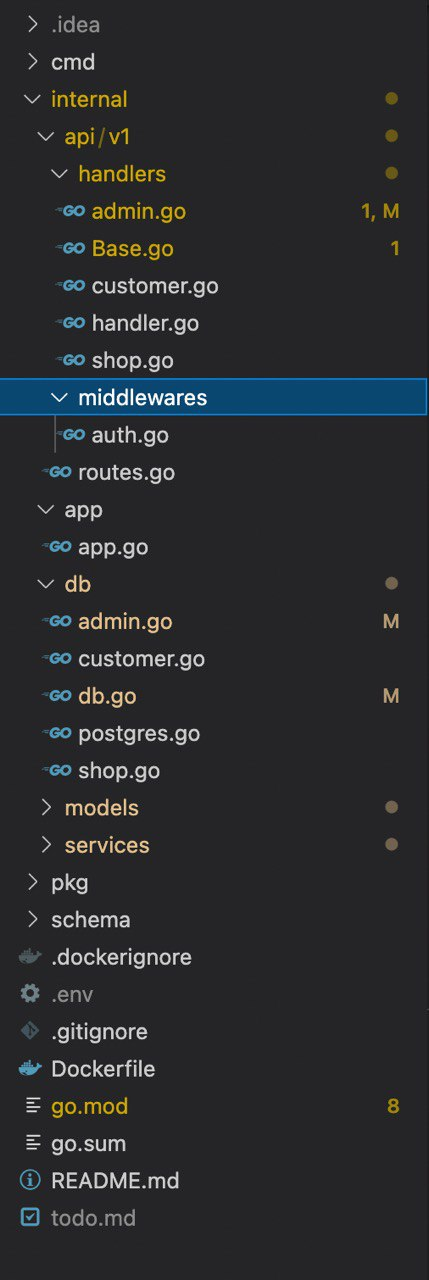
\includegraphics[scale=0.7]{figures/backend1.jpg}
    \caption{Structure of the project}
    \label{fig:backend1}
\end{figure}

We used a clean architecture, it makes the system easy to learn, simplifies development, deployment on the server, as well as maintenance of the software system. And most importantly, it gives flexibility and the opportunity to continue to have as many options as possible. Handlers provide communication with internal and external layers. (See Figure \ref{fig:backend2}). At the service level, we implement business rules, or rather, all cases of using the system. To do this, we use entities from the model level. The db folder serves as an external layer, it consists of a database and its details In the models folder, we have entities that are defined by business rules and that represent a set of data structures.
\begin{figure}[ht!]
    \centering
    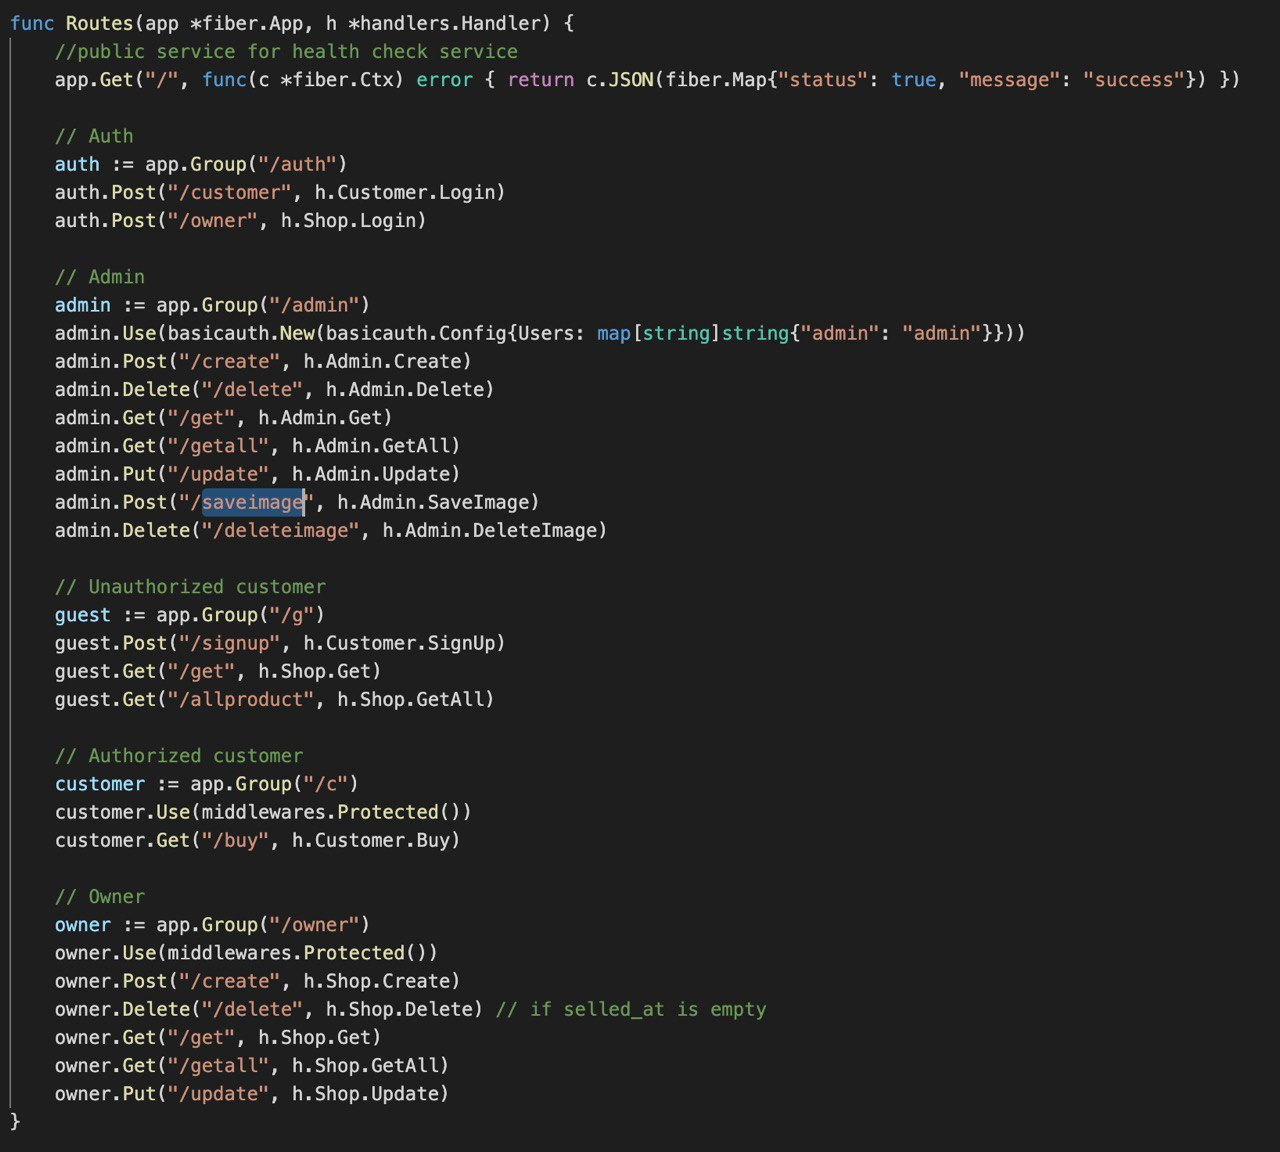
\includegraphics[scale=0.7]{figures/backend2.jpg}
    \caption{Handlers}
    \label{fig:backend2}
\end{figure}
\clearpage

\section{Front-end implementation}
This project's user section is for anyone who wants to buy old stuff. Ordinary users do not have access to the administrative section. We have numerous pages in the user section that differ in terms of information and functions. The main page of our site consists of search functions, as well as various information.(See in Figure \ref{fig:front-end})
\begin{figure}[h!]
    \centering
    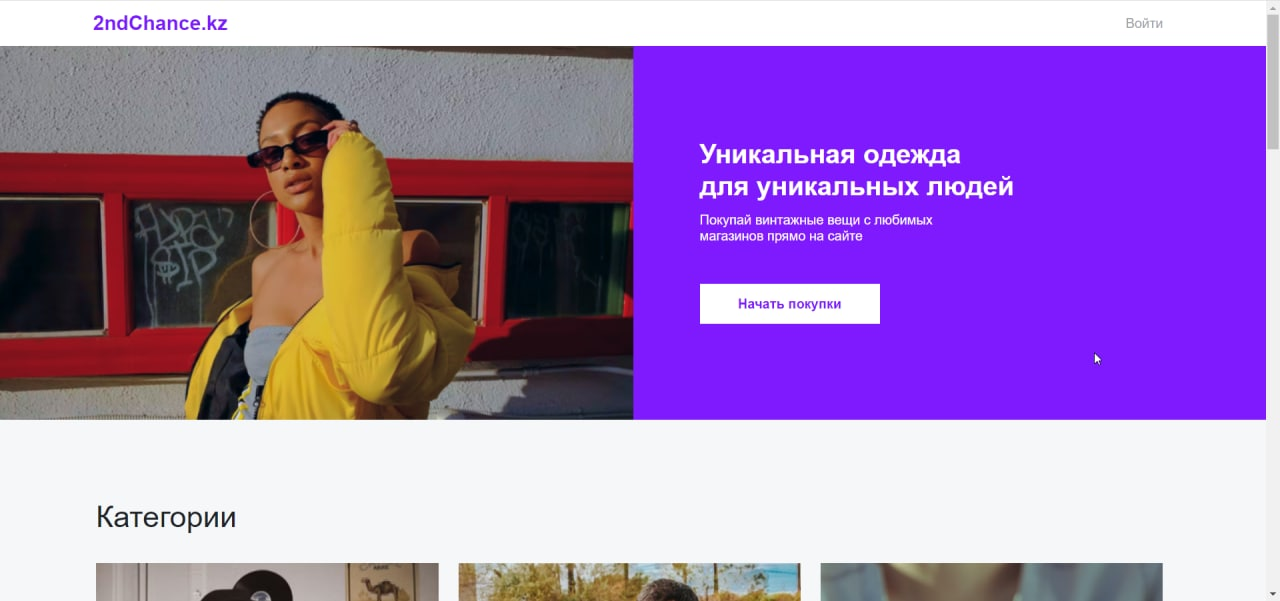
\includegraphics[scale=0.6]{figures/front-end.jpg}
    \caption{Main-page}
    \label{fig:front-end}
\end{figure}

Such as: categories, discounts of the day, auctions, shops. There are also pages such as a catalog, product details and a payment page. Several libraries were used in the creation of this site, and one of them is the most up-to-date bootstrap library. The entire front-end site was written in react js.React - JavaScript library, which helps to build UI part. Since, it's flexible and has great performance\cite{react}.

Our product site consists of two parts: user and seller. Vendors are second hand stores. They can list their products and manage them. And the client part is for users and buyers. They have the opportunity to look and buy things.
